\chapter{The Central Limit Theorem}
\label{ch:central-limit-theorem}

In this chapter the central limit theorem in introduced (cfr. Section~\ref{sec:central-limit-theorem}). This theorem is a key concept in probability theory, because multiple statistical testing procedures (cfr. Chapter~\ref{ch:testing_procedures}) are based on this. The central limit theorem allows you to generalize measurements obtained from a sample to the full population under certain conditions.

We also discuss the concept of point estimators and confidence intervals. A point estimator is a number that is calculated from the sample, which can be used to estimate a property of the population. For example, the mean/average of a sample $\overline{x}$ is a point estimator for the mean/average of the population $\mu$. A confidence interval is used to propose a range of plausible values for an unknown parameter together with an associated confidence level. For example, a 95\% confidence interval for the mean of a population is an interval derived from the sample, of which we can say that - under clear conditions - the population mean has a 95\% chance to be in the proposed range.

But before introducing these concepts, we first start with a short rehearsal of general concepts of the probability theory (cfr. Section~\ref{sec:probability-distribution-sample}) and discuss the normal distribution (cfr Section~\ref{sec:normal-distribution}).

\section{Learning Goals}
\label{sec:central-limit-theorem-learning-goals}

By the end of this chapter you must be able to:

\begin{itemize}
  \item Explain and apply the following concepts:
  \begin{itemize}
    \item Sample Space (universum), event, probability space, probability, discrete/continuous probability distribution
    \item Point Estimator, confidence interval
    \item Degrees of freedom
  \end{itemize}
  \item Sketch the probability distribution of the normal distribution for a given mean and standard deviation (Gaussian curve) and indicate the mean and standard deviation on this graph;
  \item Calculate the $z$ score of a value in a normally distributed random variable;
  \item Calculate the left- ($P(X<x)$) and right tail-probability ($P(X>x)$) or combinations of both (eg. $P(x<X<y)$) for a value in a normally distributed calculate stochastic variable, using the symmetry rule and the 100\% rule where necessary;
  \item Determine to what extent a given stochastic variable is normally distributed based on the probability density curve, QQ plot, skewness or kurtosis;
  \item Formulate the central limit theorem (and in particular know the probability distribution of the sample mean) and explain its importance for statistical analysis.
  \item Calculate a confidence interval for the population mean of a sample with a given confidence level in the following cases:
  \begin{itemize}
    \item a large sample with known population variance
    \item a small sample with unknown population variance
    \item a sampling fraction
  \end{itemize}
\end{itemize}

\section{Probability Distribution of a Sample}
\label{sec:probability-distribution-sample}

\subsection{Stochastic Experiment}
A random (or stochastic) experiment requires the following elements:

\begin{definition}[Sample Space or Universum]\
   The sample space or universum of an experiment
   is the collection of all possible outcomes of this experiment and
   is denoted by $\Omega$.
   \end{definition}

   \textbf{Remarks}
   \begin{itemize}
   \item The sample space needs to be \emph{complete} or \emph{collectively exhaustive}\/: 
   Every possible outcome of an experiment should be an element of $\Omega$.
   \item Additionally, it needs to be \emph{mutually exclusive}\/:
   Every outcome of an experiment should correspond with \emph{exactly one} element of $\Omega$.
   \item In summary: after executing an experiment it should be unambiguous 
   to indicate what element of $\Omega$ has occured.
   \end{itemize}
   
   \begin{definition}[Event]
    An \emph{event}\index{event} is a subset of the sample space. A singular or elementary event is a singleton. A composite event has a cardinality greater than 1.
\end{definition}

When $A$ and $B$ are events, the following events can be formed:
\begin{itemize}
    \item $A$ \textbf{or} $B$, noted as $A \cup B$;
    \item $A$ \textbf{and} $B$, noted as $A \cap B$;
    \item \textbf{not} $A$, noted as $\overline{A}$.
\end{itemize}

Events that don't have common outcomes are called \emph{disjoint}\index{event!disjoint}.
Consequently, disjoint events can never occur simultaneously. 
When events $A$ and $B$ are disjoint, then $A \cap B = \emptyset$. 

\textbf{Remarks}
\begin{itemize}
   \item It can be proven by induction that the union of $n$ events $A_1$ up to $A_n$ is also an event.
   \item The same goes for the intersection between events.
   \item For some application, countable infinite unions or intersections are also considered.
\end{itemize}
   
\begin{definition}[Probability space] 
    The probability of an event $A$ is noted as $P(A)$. Probabilities of events should meet the following requirements:

   \begin{enumerate}
   \item Probabilities of events are positive: $\forall A \subset \Omega: P(A) \geq 0$
   \item The total probability of all elements in $\Omega$ is 1: $P(\Omega) = 1.$
   \item If $A$ and $B$ are \emph{disjoint} events, then:
    \[P(A\cup B) = P(A) + P(B). \]
    This is called the Rule of Sum.
   \end{enumerate}

   When the probability function $P$ meets these requirements (axioms), 
   then the triple $(\Omega, \mathcal{P}(\Omega), P)$ is a \emph{probability space}\index{probability space} 
   (with $\mathcal{P}(\Omega)$ the \emph{power set} of $\Omega$, i.e.~the set of all its subsets).
\end{definition}
   
\begin{example}
\label{ex:dice}
    Consider a sample space $\Omega =  \left\{ 1,2,3,4,5,6 \right\} $ and a probability function $P(\omega) = \frac{1}{|\Omega|}$. 
    This combination could represent a dice with 6 sides, and outcomes $1, \ldots, 6$, each having a probability $P(\omega) = \frac{1}{6}$.
\end{example}
   
In this part of the syllabus we will look at \textbf{statistical inference}: make statements about the population based on a drawn sample.

\subsection{Probability distribution}
\label{ssec:probability-distribution}
   
\subsubsection{Discrete probability distribution}

If we continue the example of rolling a dice (cfr Example~\ref{ex:dice}), the probability of each outcome $\Omega = \{1,2,3,4,5,6\}$ can be summarized using a table or histogram (cfr. Figure~\ref{fig:probabilities-1-dice}). Some important notes:

\begin{enumerate}
    \item All probabilities are nonnegative.
    \item The probability of a specific outcome equals the area of the corresponding bar.
    \item The total area of all bars is 1.
\end{enumerate}

\begin{figure}
    \centering
    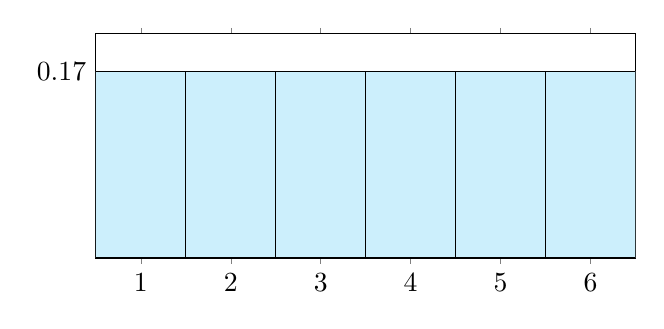
\begin{tikzpicture}
    \begin{axis}[ybar,ytick=data,ymin=0, ymax=.2, anchor=north, bar width=1, yscale=.5]
    \addplot[fill=cyan!20]
    coordinates {
        (1, 1/6)
        (2, 1/6)
        (3, 1/6)
        (4, 1/6)
        (5, 1/6)
        (6, 1/6)};
    \end{axis}
    \end{tikzpicture}
    \caption{Probability distribution when rolling a single dice.}
    \label{fig:probabilities-1-dice}
\end{figure}

When rolling \emph{two} dice, there are $6 \times 6 = 36$ possible outcomes, but some of them are equivalent. 
For example, $5$ and $2$, $2$ and $5$, $3$ and $4$, etc. all have a total outcome of $7$. 
There are two ways to roll a $3$. Consequently, $P(X=3) = \frac{2}{36}$. 
For $n = 1, \ldots, 7$, it holds that $P(X=n) = \frac{n-1}{36}$. 
Figure~\ref{fig:probabilities-2-dice} shows the corresponding histogram of the probability distribution.

\begin{figure}
    \centering
    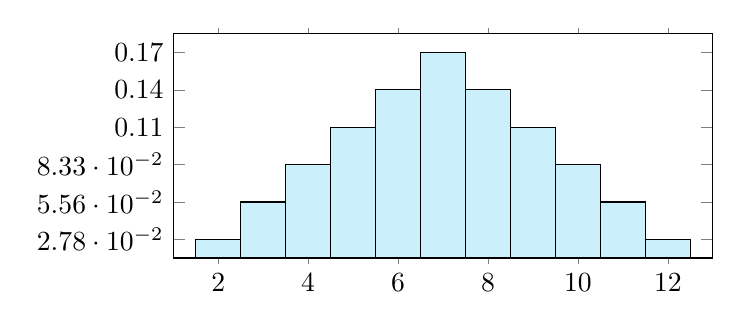
\begin{tikzpicture}
    \begin{axis}[ybar,ytick=data, anchor=north, bar width=1, yscale=.5]
    \addplot[fill=cyan!20]
    coordinates {
      (2, 1/36)
      (3, 2/36)
      (4, 3/36)
      (5, 4/36)
      (6, 5/36)
      (7, 6/36)
      (8, 5/36)
      (9, 4/36)
      (10, 3/36)
      (11, 2/36)
      (12, 1/36)
    };
    
    \end{axis}
    \end{tikzpicture}
    \caption{Probability distribution when rolling two dice.}
    \label{fig:probabilities-2-dice}
  \end{figure}

The histogram allows for the following calculations:
\begin{itemize}
  \item The probability of rolling a 10 or higher is the sum of the area of bars 10, 11, and 12.
  \item The probability of rolling a number between 2 and 7 (not included) is the sum of the area of bars 3, \ldots, 6.
  \item $\ldots$
  \item The total area is 1: the probability that 1 of all these outcomes occurs is 100\%.
\end{itemize}

\subsubsection{Continuous probability distribution}

Continuous probability distributions\index{probability distribution!continuous} are distributions where the sample space doesn't merely consist of a limited number of outcomes (nominal or ordinal level of measurement), but where outcomes can be any numeric value (interval and ratio level).
Take for example the weight of our superheroes: this is a continuous variable since a value can be not only a whole number like $70$ kg or $95$ kg, but also (approximately) $86,8735485653$ kg. In principle, any real value is possible, although in practice it's impossible to measure this exactly. This has an important consequence for the probability distribution. The distribution no longer consist of separate bars, but has become a continuous curve (cfr. Figure~\ref{fig:verdelingReactievermogen}). This implies that the probability of measuring exactly $70$ kg is effectively zero. However, when we say $70$ kg, we usually mean any value between $69.5$ and $70.5$ kg, or more precisely the interval $[69.5, 70.5[$. Likewise, $70,00000$ kg could refer to a value within the interval $[69.999995, 70.000005[$ kg.

The properties of probability distributions mentioned before still hold. The surface below the curve totals to 1. Also, the probability between two values is the surface below the curve, between the boundaries defined by these values. Remark that it's not actually important whether the limits are included or not, since their probabilities are negligable.

\section{The normal distribution}
\label{sec:normal-distribution}

\begin{figure}[t]
\centering
\begin{tikzpicture}
\begin{axis}[
  domain=0:10, samples=100,
  axis lines*=left, xlabel=$x$, ylabel=$y$,
  every axis y label/.style={at=(current axis.above origin),anchor=south},
  every axis x label/.style={at=(current axis.right of origin),anchor=west},
  height=5cm, width=12cm,
  xtick={5,3.5,6.5}, ytick=\empty,
  enlargelimits=false, clip=false, axis on top,
  grid = major
  ]
  \addplot [fill=cyan!20, draw=none, domain=0:9] {gauss(5,1.5)} \closedcycle;
  \draw [yshift=-0.6cm, latex-latex](axis cs:3.5,0) -- node [fill=white] {$\sigma$} (axis cs:5.0,0);
\end{axis}
\end{tikzpicture}
\caption{The probability of Superman's reaction speed. This curve illustrates the normal distribution with mean $\mu = 5$ ms and standard deviation $\sigma = 1.5 ms.$}
\label{fig:verdelingReactievermogen}
\end{figure}


Figure \ref{fig:verdelingReactievermogen} illustrates the probability distribution of Superman's reaction speed, variable $X$. The curve follows the normal distribution\index{distribution!normal} with a mean of 5 ms and a standard deviation of 1.5 ms. This is also notated as:
\[ X  \sim Nor(\mu = 5; \sigma = 1.5) \]

The equation of this function, the probability density, is sometimes referred to as the Gaussian bell curve, called after mathematician Carl Friedrich Gauss:
\begin{equation}
  f(x) = \frac{1}{\sigma \sqrt{2\pi}} e^{-\frac{1}{2} \frac{(x - \mu)^{2}}{\sigma^{2}}}
  \label{eq:normalFunction}
\end{equation}

De normal distribution has the following properties:
\begin{itemize}
  \item The probability density is bell-shaped;
  \item The probability density is symmetric around $\mu$;
  \item Because of this symmetry, the mean, median and mode are equal;
  \item The total area below the bell curve and above the $x$-axis is 1;
  \item The area between $\mu - \sigma$ en $\mu + \sigma$ (the so-called sigma area) contains approximately 68\% of the observations;
  \item The area between $\mu - 2 \sigma$ and $\mu + 2 \sigma$ contains about 95\% of all observations;
  \item The area between $\mu - 3 \sigma$ and $\mu + 3 \sigma$ contains about 99.7\% of all observations;
  \item The different areas are illustrated in Figure~\ref{fig:standard-normal-distribution}.
\end{itemize}

\subsection{The standard normal distribution}
\label{ssec:standard-normal-distribution}

If the distribution of stochastic variable $X$ is $X \sim N(\mu, \sigma)$, then the distribution of $Z = \frac{X - \mu}{\sigma}$ is $Z \sim N(0,1)$. This is called the standard normal distribution\index{distribution!standard normal}.

% Bron: http://johncanning.net/wp/?p=1202
\begin{center}
\begin{figure}
\centering
\begin{tikzpicture}
    \begin{axis}[
        no markers, domain=0:10, samples=100,
        axis lines*=left,height=6cm, width=10cm,
        xtick={-3, -2, -1, 0, 1, 2, 3}, ytick=\empty,
        enlargelimits=false, clip=false, axis on top,
        grid = major
    ]
    \addplot [smooth,fill=cyan!20, draw=none, domain=-3:3] {gauss(0,1)} \closedcycle;
    \addplot [smooth,fill=orange!20, draw=none, domain=-3:-2] {gauss(0,1)} \closedcycle;
    \addplot [smooth,fill=orange!20, draw=none, domain=2:3] {gauss(0,1)} \closedcycle;
    \addplot [smooth,fill=blue!20, draw=none, domain=-2:-1] {gauss(0,1)} \closedcycle;
    \addplot [smooth,fill=blue!20, draw=none, domain=1:2] {gauss(0,1)} \closedcycle;
    \addplot[<->] coordinates {(-1,0.4) (1,0.4)};
    \addplot[<->] coordinates {(-2,0.3) (2,0.3)};
    \addplot[<->] coordinates {(-3,0.2) (3,0.2)};
    \node[coordinate, pin={68.3\%}] at (axis cs: 0, 0.35){};
    \node[coordinate, pin={95.4\%}] at (axis cs: 0, 0.25){};
    \node[coordinate, pin={99.7\%}] at (axis cs: 0, 0.15){};
    \node[coordinate, pin={34.1\%}] at (axis cs: -0.5, 0){};
    \node[coordinate, pin={34.1\%}] at (axis cs: 0.5, 0){};
    \node[coordinate, pin={13.6\%}] at (axis cs: 1.5, 0){};
    \node[coordinate, pin={13.6\%}] at (axis cs: -1.5, 0){};
    \node[coordinate, pin={2.1\%}] at (axis cs: 2.5, 0){};
    \node[coordinate, pin={2.1\%}] at (axis cs: -2.5, 0){};
    \end{axis}
\end{tikzpicture}
\caption{The standard normal distribution with different ``zones'' indicating the percentage of observations within each zone.}
\label{fig:standard-normal-distribution}
\end{figure}
\end{center}

Often, it is useful to compare observations from different normal distributions. We can \emph{normalize} an observation by calculating the distance from the mean in terms of the standard deviation. This is called the $z$-score and is calculated as follows:

\begin{equation}
    z = \frac{x-\mu}{\sigma}
    \label{eq:zscore}
  \end{equation}

This score indicates how extreme an observation is, or in other words how many standard deviations it is located away from the mean. 
For a random value of $x$ we can use Equation~\ref{eq:zscore} to calculate the corresponding $z$-score.
The $z$-scores are so significant and often used that specific tables were composed containing the probabilities that an observation drawn from $Z$ is smaller than $z$, the so-called left tail probability\footnote{Similar tables containing the right tail probability exist as well}: $P(Z<z)$.

R also has functions for calculating with probabilities of normally distributed variables. These are summarized in Table~\ref{rab:norm-prob-r}.

\begin{table}
  \centering
  \begin{tabular}{ll}
  	\textbf{Function}     & \textbf{Description}                                           \\ \hline
  	\verb|pnorm(x, m, s)| & Left tail probability, $P(X<\mathtt{x})$                       \\
  	\verb|dnorm(x, m, s)| & Altitude of the Gaussian curve at point \texttt{x}             \\
  	\verb|qnorm(p, m, s)| & What boundary value contains \texttt{p}\% of the obversvations?\\
  	\verb|rnorm(n, m, s)| & Generate\texttt{n} normally distributed random numbers
  \end{tabular}

  \caption{Functions for calculating the probability in R for a normal distribution with average \texttt{m} and standard deviation \texttt{s}. If the value for arguments \texttt{m} and \texttt{s} are omitted, the standard normal distribution is used.}
  \label{rab:norm-prob-r}
\end{table}

In order to calculate probabilities for any normal distribution, the following method can be used:

\begin{enumerate}
  \item Determine the stochastic variable with the associated normal distribution ($\mu$ and $\sigma$);
  \item Calculate the $z$-score for a given $x$-value;
  \item Reduce the requested probability to a left tail probability, using the probabilities of the normal distribution:
  \begin{itemize}
    \item $P(Z > z) = P(Z < -z)$ (symmetry rule);
    \item $P(Z > z) = 1 - P(Z < z)$ (100\% probability rule)
  \end{itemize}
\end{enumerate}

Plotting or sketching the requested probability is also very useful to gain insight into the calculation.

\begin{example}
What is the probability that Superman reacts in less than 4 ms?
\[ P(X < 4) = P(Z < -0,67) = 0,2514 \]
\end{example}

\begin{example}
What is the probability that he reacts in less than 7 ms?
\[ P(X < 7) = P(Z < 1,33) = 0,9082 \]
\end{example}

\begin{example}
What is the probability that he reacts in less than 3 ms?
\[ P(X<3) = P(Z < -1,33) = 0,0918 \]
\end{example}

\begin{example}
What is the probability that he reacts between 2 en 6.5 ms?
\[ P( 2 < X < 6,5) = P(X<6,5) - P(X<2) = P(Z<1) - P(Z<-2) = 0,8186 \]
\end{example}

\subsection{Testing for normality}
\label{ssec:testing-for-normality}

Because of the desirable properties of the normal distribution, it's often good to know whether a sample is actually drawn from a normal distribution. Several methods exist to test for normality:

\begin{enumerate}
  \item Plot a histogram for the data and look at the shape of the chart. If the observations are drawn from a normal distribution, the shape will approximate a bell curve.
  \item Calculate the intervals $\overline{x} \pm s$, $\overline{x} \pm 2s$, $\overline{x} \pm 3s$ and determine the percentage of observations in each interval. If the observations are normally distributed, these percentages should be around 68\%, 95\%, and 99,7\%, respectively.
  \item Draw a Q-Q plot\index{Q-Q plot} (normality plot, cfr. Definition~\ref{def:qq-plot}) for the observations. If they are normally distributed, the observations will be plotted approximately on a straight line.
  \item Calculate the \emph{kurtosis}\index{kurtosis}, a metric for the ``sharpness'' of the distribution's ``peak'':
    \begin{itemize}
      \item A normal distribution has a kurtosis of 3, or, alternatively, an \emph{excess kurtosis}\index{kurtosis!excess} of 0;
      \item A ``flat'' distribution has a negative excess kurtosis;
      \item A distribution with a sharp peak has a positive excess kurtosis.
      \item Note: when using the original definition of kurtosis, the normal distribution has a kurtosis of 3. We however use an alternative definition of kurtotis here, often referred to as the ``excess kurtosis'', which substracts 3 of the original value, resulting in a kurtosis of 0 for a normal distribution.
    \end{itemize}
  \item Calculate the \emph{skewness}\index{skewness}, a metric for the symmetry of the data:
    \begin{itemize}
      \item A symmetric distribution (including the normal distribution) has a skewness of 0;
      \item A distribution with a long left tail has a negative skewness;
      \item A distribution with a long right tail has a positive skewness;
      \item Rule of thumb: if the absolute value of the skewness $>1$, the distribution is not considered to be symmetrical.
    \end{itemize}
\end{enumerate}

\begin{definition}[Q-Q plot or normality plot]
    \label{def:qq-plot}
    A normality plot, or \emph{Q-Q plot}\index{Q-Q plot}\footnote{Q stands for quantile} for a set of observations is a probability plot with the sorted observations on one axis and the associated expected $z$-values on the other axis. See Figure~\ref{fig:qqplot} for some examples. The code in R used for generating the images is given below. If the data is normally distributed, the observations will be plotted on or near the line $y = x$.
  \end{definition}

\begin{figure}
  \begin{center}
    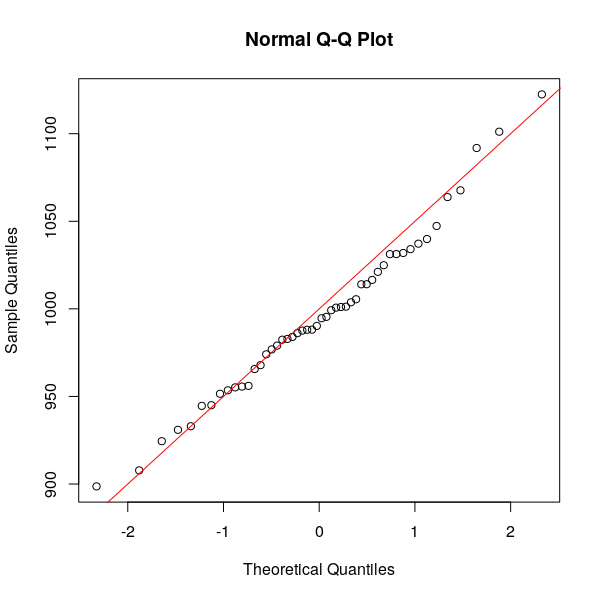
\includegraphics[width=.45\textwidth]{sampling-qqplot-good}
    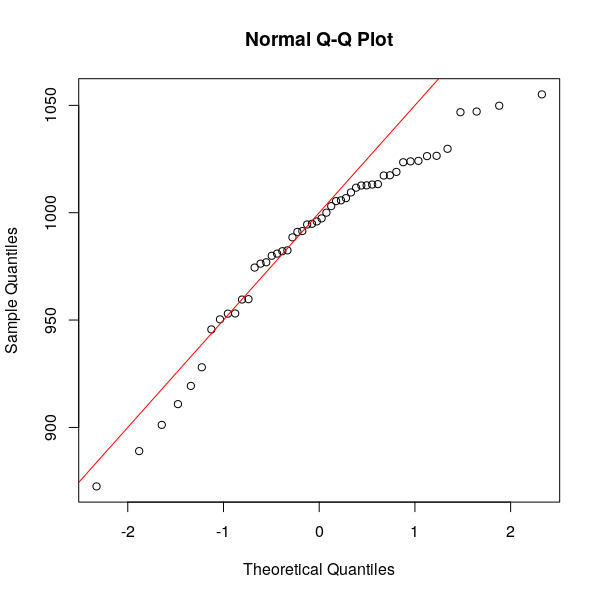
\includegraphics[width=.45\textwidth]{sampling-qqplot-bad}
  \end{center}
  \caption{The Q-Q plot on the left is based on a sample of 50 observations drawn from a normal distribution with mean 1000 and standard deviation 50. The plot on the right is based on a sample of 50 observations drawn from Student's $t$ distribution with 15 degrees of freedom, with the same mean and standard deviation. The lines in red indicate where the observations should theoretically be situated. In the plot on the left, this is more or less the case, but on the right, especially in the extremes, observations deviate from the line.}
  \label{fig:qqplot}
\end{figure}

\lstinputlisting{data/qqplot.R}

\section{The Central Limit Theorem}
\label{sec:central-limit-theorem}

In this section, we'll discuss one of the most fundamental results in statistics and the foundation of sampling: the central limit theorem.

\begin{definition}[Linear combination of independent, identically distributed stochastic variables]
  Formal: A linear combination of a sufficiently large number of independent, identically distributed stochastic variables (i.e. with a well defined expected value and variance) will approximate the normal distribution, regardless of the underlying distribution.

  \[X_{i} \sim Nor(\mu_{i}, \sigma_{i}) \Rightarrow Y = \sum_{i} \alpha_{i} X_{i} \textnormal{ approximates the normal distribution} \]

  Consequently, the mean of a sample derived from a population with a random distribution will approximate a normal distribution for a sufficiently large value of $n$.
\end{definition}

Therefore, given a random sample of independent variables with a normal distribution,
the central limit theorem states that the mean of this sample will also approximate the normal distribution.
So, if you would repeatedly take a sample of the same size, and measure the mean, the resulting plot will approximate the graph of a normal distribution (cfr. Figure~\ref{sec:normal-distribution}).
The larger the sample, the closer the approximation will be.
The mean of the sample therefore has a normal distribution, independent of the underlying distribution of the metric from which a sample is taken. 

In general:

\begin{definition}[The Central Limit Theorem]
  Consider a random sample of $n$ observations drawn from a population with expected value $\mu$ and standard deviation $\sigma$.
  If $n$ is sufficiently large, the probability distribution of the sample mean $\overline{x}$ will approximate a normal distribution with expected value $\mu_{\overline{x}} = \mu$ and standard deviation $\sigma_{\overline{x}} = \frac{\sigma}{\sqrt{n}}$.
  The larger the sample, the better the probability distribution of $\overline{x}$ will approximate the expected value of the population, $\mu$.
\end{definition}

When taking a sample, the underlying distribution is rarely known, and yet one can make statements about the sample mean. This is entirely thanks to the central limit theorem, which imposes a rule about the mean regardless of the underlying probability distribution. 
The central limit theorem keeps the sample mean under control, locking it in the Gaussian cage from which it can never escape. This, and only this, allows scientists to study it carefully, observe it, and enables them to formulate conclusions.

Because, if the distribution of the sample mean would depend on the underlying distribution, which would be expected to some extent, it would be impossible to make concrete statements about many scientific results. 
In statistics theory, limits of sample means appear everywhere, and they can be easily replaced by a normal distribution thanks to the central limit theorem. 
If this would not be possible, the whole theory of estimating parameters would collapse, which would be disastrous in practice. 
Comparing research would be reduced to an almost impossible task, and statistics in general would become much more difficult and complicated.

The proof of the central limit theorem is outside the scope of this course, even though it is surprisingly easy to understand.

\subsection{Application of the Central Limit Theorem}
When drawing a random sample of a sufficiently large size $n$ form a population with an unknown $\mu$ and (known) standard deviation $\sigma$, the probability distribution of the sample mean is a stochastic variable $M \sim N (\overline{x}, \frac{\sigma}{\sqrt{n}})$.

\begin{example}
  Let's consider the reaction times of all our superheroes and assume we have drawn a random sample with $n = 100$, $\overline{x} = 90, and \sigma = 60$ (ms).
  We can then ask ourselves: what is the probability that the average reaction time of a superhero is below $104$ ms?

  \begin{enumerate}
    \item In this example, the stochastic variable is the average reaction speed $\overline{x}$ in a sample of $n=100$ superheroes. Because of the central limit theory, the following holds:
    \[ \overline{x} \sim Nor(\mu = 90, \sigma_{\overline{x}} = \frac{60}{\sqrt{100}} = 6) \]
    \item We can calculate the associated $z$-score:
    \[ z = \frac{104-90}{\frac{60}{\sqrt{100}}} = \frac{104-90}{6} = 2.33 \]
    \item And therefore: $P(\overline{x} < 104) = P(Z < 2.33) = 1 - 0.0099 \approx 0.99$ or about 99\%
  \end{enumerate}
\end{example}

\subsection{Estimating Stochastic Parameters}
\label{ssec:estimating-stochastic-parameters}

If we want to study a sample, it is usually to draw conclusions about the population as a whole. 
For example, we want to know the average strength of a superhero, or the fraction of rich superheroes. 
In general, we'll \emph{estimate} a parameter of the population based on the sample. For example, $\overline{x}$ is used as an estimate of $\mu$. This type of estimation is defined as:

\begin{definition}[point estimate]
  A \emph{Point Estimate}\index{estimate!point} for a population parameter is a formula or equation that allows us to calculate a value to estimate that parameter.
\end{definition}

Another type of estimates are \emph{interval estimates}\index{estimate!interval}, a.o.~confidence intervals. These are discussed in the next sections.

\subsection{Confidence interval for the population mean of a large sample}
\label{ssec:confidence-interval-pop-mean-large-sample}

When we estimate the population mean from a sample, we have no idea how correct this estimate is. However, the properties of the normal distribution allow us to construct an interval that will contain the population mean with the desired level of confidence.

\begin{definition}[Confidence Interval]
  A \emph{Confidence Interval}\index{confidence interval} is an equation or formula that allows us to construct an interval that will contain the parameter to be estimated with a certain level of confidence.
\end{definition}

An initial estimate for the population mean is of course the sample mean:

\[ \overline{x} = \frac{1}{n} \sum_{i} x_{i} \]

Of course this estimate is not the real population mean. However, because of the central limit theorem, we know that the mean of a sample of size $n$ is normally distributed with mean $\mu$ and standard deviation $\frac{\sigma}{\sqrt{n}}$.
After standardisation, we get:
\[ Z = \frac{\overline{x} - \mu}{\frac{\sigma}{\sqrt{n}}} \]

This expression depends on $\mu$, but we know that this parameter has a normal distribution. As a result, we can find limits $-z$ and $z$, independent from $\mu$, that will contain $Z$ with a \emph{confidence level} $1 - \alpha$ (which can be chosen by the researcher). In this example, we choose $1 - \alpha= 0.95$ (and consequently $\alpha = 0.05$).

\[P(-z < Z < z) = 1 - \alpha = 0.95 \]

After applying the rule of symmetry, we find that we need to determine $z$ by:

\[ P( Z < z) = 1 - 0,025 = 0.975 \]

When we look this up in a Z-table, we'll find that $z = 1.96$. Or, alternatively, we can calculate \verb|qnorm(0.975)| in R.

The confidence interval then is:

\[ P( -1.96 < \frac{\overline{x} - \mu}{\frac{\sigma}{\sqrt{n}}} < 1.96 ) = 1 - \alpha\]

and therefore
\[ P ( \overline{x} -1.96 \frac{\sigma}{\sqrt{n}} <\mu < \overline{x} + 1.96 \frac{\sigma}{\sqrt{n}}) = 1 - \alpha \]

Using this technique, we can determine the bounds of an interval that will contain $\mu$ with a confidence level of 95\%. 
If you would repeatedly draw a sample from this population and calculate the confidence interval around $\overline{x}$, then in 95\% of the cases, we expect the actual $\mu$ to be inside the interval bounds.

However, note that we assume to know the standard deviation of the population, which will generally not be the case. If the sample size is sufficiently large, the standard deviation of the sample is used as a point estimate for the standard deviation of the population.

\[ P ( \overline{x} -1,96 \frac{\sigma_{\overline{x}}}{\sqrt{n}} < \mu < \overline{x} + 1,96 \frac{\sigma_{\overline{x}}}{\sqrt{n}}) = 1 - \alpha \]


\begin{figure}
\centering
\begin{tikzpicture}
\begin{axis}[
  domain=-3:3, samples=100,
  axis lines*=left, xlabel=$z$,
  every axis y label/.style={at=(current axis.above origin),anchor=south},
  every axis x label/.style={at=(current axis.right of origin),anchor=west},
  height=5cm, width=12cm,
  xtick={-1.96,0,1.96}, ytick=\empty,
  enlargelimits=false, clip=false, axis on top,
  grid = major
  ]
  \addplot [fill=cyan!20, draw=none, domain=-3:3] {gauss(0,1)} \closedcycle;
  \draw [yshift=-0.6cm, latex-latex](axis cs:-1.96,0) -- node [fill=white] {$\sigma$} (axis cs:1.96,0);
\end{axis}
\end{tikzpicture}
\caption{Standard normal distribution with a 95\% confidence interval.}
\label{fig:verdelingStandaardnormaal}
\end{figure}

\subsection{Confidence interval for the population mean of a small sample}
\label{ssec:confidence-interval-pop-mean-small-sample}

Bij kleine steekproeven kunnen we niet langer veronderstellen dat de kansverdeling van $\overline{x}$ bij benadering
normaal verdeel is, omdat de centrale limietstelling alleen normaliteit garandeert voor grote steekproeven ($n >30$). De vorm
van de kansverdeling van het steekproefgemiddelde $\overline{x}$ hangt nu af van de vorm van de verdeling van de populatie waaruit de
steekproef genomen wordt. Alhoewel nog steeds geldt dat $\sigma_{\overline{x}} = \frac{\sigma}{\sqrt{n}}$ kan
de standaardafwijking $s$ een slechte benadering zijn voor $\sigma$ als de steekproef klein is.

Als oplossing kunnen we een nieuwe grootheid bepalen. In plaats van

\[ z = \frac{\overline{x} - \mu}{\frac{\sigma}{\sqrt{n}}} \]

construeren we

\[ t = \frac{\overline{x} - \mu}{\frac{s}{\sqrt{n}}} \]

Deze heeft een kansverdeling die beschreven wordt door een Student-t verdeling. Deze lijkt zeer goed op de normale verdeling: klokvormig, symmetrisch en met verwachtingswaarde 0.

De precieze vorm van de kansverdeling $t$ hang af van de steekproefomvang $n$. We zeggen dat de t-verdeling $(n-1)$ vrijheidsgraden heeft (afgekort $df$).
Merk op dat:
\begin{itemize}
  \item $(n-1)$ ook gebruikt werd om $s^{2}$ te berekenen
  \item als $n \rightarrow \infty$ we de standaardnormale verdeling verkrijgen.
\end{itemize}

Indien we nu een betrouwbaarheidsinterval willen bepalen voor een steekproef met een klein aantal waarden moeten we het volgende doen:

\begin{definition}[Betrouwbaarheidsinterval kleine steekproef]
  Om een betrouwbaarheidsinterval voor het gemiddelde te bepalen op basis van een klein steekproef bepalen we:
  \[ \overline{x} \pm t_{\frac{\alpha}{2}}(\frac{s}{\sqrt{n}}) \]
  waarbij $t_{\frac{\alpha}{2}}$ gebaseerd is op $(n-1)$ vrijheidsgraden. We veronderstellen wel dat we een aselecte steekproef genomen hebben uit
  een populatie die bij benadering normaal verdeeld is.
\end{definition}

\begin{table}
  \centering
  \begin{tabular}{ll}
  	\textbf{Functie} & \textbf{Betekenis}                                             \\ \midrule
  	\verb|pt(x, df)| & Linkerstaartkans, $P(X<\mathtt{x})$                            \\
  	\verb|dt(x, df)| & Hoogte van de curve op punt \texttt{x}                         \\
  	\verb|qt(p, df)| & Onder welke grens zal \texttt{p}\% van de waarnemingen liggen? \\
  	\verb|rt(n, df)| & Genereer \texttt{n} random getallen volgens deze verdeling
  \end{tabular}

  \caption{Kansberekeningsfuncties in R voor de Student-$t$ verdeling met \texttt{df} vrijheidsgraden, verwachte waarde 0 en standaardafwijking 1.}
  \label{tab:t-prob-r}
\end{table}

\subsection{Betrouwbaarheidsinterval voor populatiefractie bij een grote steekproef}
\label{ssec:betrouwbaarheidsinterval-populatiefractie}

Indien je een variabele wil meten als een fractie, bijvoorbeeld \% mensen die ja geantwoord heeft op een bepaalde vraag, dan willen we in feite de kans $p$ op succes in een bernouilli experiment schatten, waarbij $p$ de kans is dat een willekeurig geselecteerde respondent (of element van de populatie) een succes is (succes in termen van binomiaal experiment). We kunnen $p$ dan schatten door bijvoorbeeld:

\[ \overline{p} = \frac{\textnormal{aantal successen}}{n} \]

Om nu de betrouwbaarheid van de schatter $\overline{p}$ te bepalen moeten we de kansverdeling kennen van $\overline{p}$. Dit kunnen we beredeneren door toepassing van de centrale limietstelling op het gemiddelde aantal successen in de steekproef van omvang $n$. Indien succes = 1 en faling = 0, dan hebben we een steekproef van $n$ elementen, ieder met dezelfde verdeling (kans op 1 is $p$ en kans op 0 is $q=1-p$).  Het gemiddelde $\overline{p}$ heeft dan bij benadering een normale verdeling. Of dus:

\begin{itemize}
  \item Verwachting van kansverdeling van $\overline{p}$ is $p$.
  \item De standaardafwijking van kansverdeling $\overline{p} = \sqrt{\frac{pq}{n}}$
  \item Voor grote steekproeven is $\overline{p}$ bij benadering normaal verdeeld.
\end{itemize}

Aangezien $\overline{p}$ een steekproefgemiddelde is van het aantal successen, stelt dit ons in staat een betrouwbaarheidsinterval te berekenen analoog als die voor de intervalschatting van $\mu$ voor grote steekproeven.

\begin{definition}[Betrouwbaarheidsinterval voor $p$ gebaseerd op grote steekproef]
  \[ \overline{p} \pm z_{\frac{\alpha}{2}} \sqrt{\frac{\overline{p}\overline{q}}{n}} \]
  met $\overline{p} = \frac{x}{n}$ en $\overline{q} = 1- \overline{p}$
\end{definition}


\section{R}
We kijken naar enkele basisoperaties die verband houden met enkele distributies. Er zijn een groot aantal verdelingen beschikbaar, maar we kijken maar naar een paar. Als u wilt weten welke distributies beschikbaar zijn, kunt u een zoekopdracht uitvoeren met behulp van de opdracht

\begin{lstlisting}
> help.search ("distribution").
\end{lstlisting}


Hier geven we details over de commando's die verband houden met de normale distributie en vermelden kort de commando's voor andere distributies. De functies voor verschillende verdelingen zijn zeer vergelijkbaar.

De prefixen zijn als volgt:
\begin{description}
	\item[d] geeft de hoogte van de respectievelijke kansdichtheidsfunctie
	\item[p] geeft de cumulatieve kansdichtheidsfunctie
	\item[q] geeft de omgekeerde cumulatieve dichtheidsfunctie
	\item[r] geeft een willekeurige waarde
\end{description}

\subsection{De normale verdeling}
Er zijn vier functies die kunnen worden gebruikt om de waarden geassocieerd met de normale distributie te genereren.
\subsubsection{dnorm}

De eerste functie waarnaar we kijken, is \texttt{dnorm}. Gegeven een waarde geeft het de hoogte van de kansverdeling op elk punt terug. Als u alleen de punten zonder gemiddelde en standaardafwijking ingeeft wordt een gemiddelde van nul en standaardafwijking van 1 beschouwd. Er zijn opties om verschillende waarden voor de gemiddelde en standaardafwijking te gebruiken.

%\lstinputlisting{data/norm.R}

\subsubsection{pnorm}

Dit is de cumulatieve kansdichtheidsfunctie, of anders gezegd de linkerstaartkans: \texttt{pnorm(x)} is $P(Z < x)$.

\subsubsection{qnorm}
De volgende functie die we bekijken is \texttt{qnorm}, die de inverse van \texttt{pnorm} is. Het idee achter \texttt{qnorm} is dat je het een kans $\alpha$ geeft, en het geeft het getal weer waarvan de cumulatieve distributie overeenkomt met de waarschijnlijkheid $\alpha$.

\subsubsection{rnorm}

%\lstinputlisting{data/qnorm.R}
De laatste functie die we onderzoeken is de \texttt{rnorm} functie die willekeurige getallen kan genereren waarvan de distributie normaal is. Het argument dat je ingeeft is het aantal willekeurige getallen dat u wilt, met optionele argumenten om de gemiddelde en standaardafwijking op te geven:

%\lstinputlisting{data/rnorm.R}

\section{Oefeningen}
\label{sec:steekproefonderzoek-oefeningen}

\begin{exercise}
  \label{ex:prob-norm-dist}
  Bereken ook elke keer het gevraagde gebied.
  \begin{enumerate}[label=\alph*.]
    \item $P(Z < 1.33)$
    \item $P(Z > 1.33)$
    \item $P(Z < -1.33)$
    \item $P(Z > -1.33)$
    \item $P(Z < 0.45)$
    \item $P(Z > -1.05)$
    \item $P(Z < 0.65)$
    \item $P(-0.45 < Z < 1.20)$
    \item $P(-1.35 < Z < -0.10)$
    \item $P(-2.10 < Z < -0.90)$
  \end{enumerate}
\end{exercise}

\begin{exercise}
	Bepaal de dichtheid en de cumulatieve waarschijnlijkheidscurve voor een normale verdeling met een gemiddelde $\mu$
	van 2,5 en $\sigma = 1,5$. Bepaal de oppervlakte voor het gebied onder de dichtheidscurve tussen
	$x = 0.5$ en $x = 4$. Controleer uw antwoord door de berekening te doen.
\end{exercise}

\begin{exercise}
	Bepaal de dichtheid en de cumulatieve waarschijnlijkheidscurve voor een t-verdeling met $df = 3$. Teken ook een normale verdeling met een $\mu = 0$  en $\sigma = 1$.
\end{exercise}

\begin{exercise}
Gebruik de functie \verb|rnorm()| een willekeurige steekproef van 25 waarden uit een normale verdeling te tekenen met een gemiddelde van 0 en een standaardafwijking gelijk aan 1,0. Gebruik een histogram, met \verb|probability = TRUE|.

Maak een overlay over het histogram met: (a) de theoretische dichtheidscurve voor een normale verdeling met gemiddelde 0 en standaardafwijking gelijk aan 1,0; (b) een ``geschatte'' dichtheidscurve op basis van het gemeten steekproefgemiddelde en -standaardafwijking.

Herhaal dit voor een steekproef van 100 en 500 waarden.
\end{exercise}

\begin{exercise}
  In de  Hogeschool zijn er twee klassen voor het vak onderzoekstechnieken. De studenten werden willekeurig over de klassen verdeeld, zodat we mogen veronderstellen dat de ene klas niet slimmer is dan de andere. In de A-klas geeft mevr. X les, in de B-klas geeft mr. Y les. X is nogal streng en op het einde van het schooljaar behaalt haar klas een gemiddelde van 54 op 100 met een standaardafwijking van 11.

  Y is iets losser en stimuleert de leerlingen al gauw met een puntje meer. Op het einde van het schooljaar behaalt zijn klas een gemiddelde van 62 op 100 en een standaardafwijking van 7.

  Wouter zit in de A-klas en heeft $\frac{63}{100}$ voor wiskunde. Stijn zit in de B-klas en behaalt $\frac{67}{100}$. Wie heeft volgens jou het beste gescoord binnen de eigen klas?
\end{exercise}

\begin{exercise}
  Een gezondheidsonderzoek tussen 1988 en 1994 gaf aan dat de gemiddelde cholesterolwaarde bij vrouwen tussen 20 en 29 jaar 183 mg/dl bedroeg, met een standaardafwijking gelijk aan 36. We nemen nu een aselecte steekproef van 81 vrouwen. Los volgende vragen op:

  \begin{enumerate}[label=\alph*.]
    \item Schets de kansdichtheidsfunctie voor de populatie en de kansverdeling van het steekproefgemiddelde $\overline{x}$.
    \item Bepaald de kans dat $\overline{x}$ kleiner is dan 185.
    \item Bepaal de kans dat $\overline{x}$ tussen 175 en 185 ligt.
    \item Bepaal de kans dat $\overline{x}$ groter is dan 190.
  \end{enumerate}
\end{exercise}

\begin{exercise}
  Een aselecte steekproef van 64 stuks wordt getrokken uit een populatie met onbekende verdeling. De verwachting en de standaardafwijking van de populatie
  zijn wel gekend: $\mu = 20$ en $\sigma=16$. Los volgende vragen op:

  \begin{enumerate}[label=\alph*.]
    \item Bepaal de verwachting en standaardafwijking van het steekproefgemiddelde.
    \item Beschrijf de vorm van de verdeling van het steekproefgemiddelde. In hoeverre hangt je antwoord af van de grootte van de steekproef?
    \item Bereken de $z$ score bij $\overline{x_{1}} = 15.5$ en $\overline{x_{2}} = 23$.
    \item Bepaal kans dat $\overline{x} <16$.
    \item Bepaal kans dat $\overline{x} > 23$.
    \item Bepaal kans dat $16< \overline{x}< 22$.
  \end{enumerate}
\end{exercise}

\begin{exercise}
  Verkeersdrempels zijn bedoeld om de snelheid van automobilisten te be\"invloeden. Afhankelijk van de gewenste snelheid in een straat worden de drempels steiler of minder steil gemaakt. Drempel A is zo ontworpen dat 85 \% van de automobilisten de drempel passeert met een snelheid van minder dan 50 km per uur. In de praktijk blijkt dat de passeersnelheid bij een drempel normaal verdeeld is. Bij drempel A werd een gemiddelde passeersnelheid van 43,1 km/h gevonden met standaardafwijking 6,6 km/h.

  \begin{enumerate}[label=\alph*.]
    \item Toon aan dat 85\% van de automobilisten niet harder dan 50 km/h rijdt.
    \item Bij hoeveel van de 1200 metingen kan, op grond van eerdere ervaringen, een snelheid van meer dan 55 km/h worden verwacht?
  \end{enumerate}
\end{exercise}

\begin{exercise}
  Een conservenfabrikant krijgt de laatste tijd klachten over de netto inhoud van zijn conserven met wortelen en erwtjes, die volgens de verpakking netto 1 liter zouden moeten bevatten. Daarom laat hij een steekproef nemen waarin de netto inhoud van 40 willekeurig gekozen blikjes wordt gecontroleerd. De resultaten worden samengevat in Tabel~\ref{tab:Steekproefwaarden}.

Vraag A:
\begin{itemize}
  \item Vul de tabel aan met de cumulatieve absolute frequentie
  \item Vul de tabel aan met de relatieve frequentie
  \item Vul de tabel aan met de cumulatieve relatieve frequentie.
\end{itemize}
Vraag B:

\begin{itemize}
  \item Bereken het gemiddelde
  \item Bereken de standaardafwijking
  \item Hoeveel procent van de blikken bevatten te weinig wortelen en erwtjes.
  \item Teken een histogram van de absolute frequentie.
  \item Zijn de gegevens normaal verdeeld?  Hoe zie je dat?
\end{itemize}

\end{exercise}

  \begin{table}
  \centering
  \begin{tabular}{lr}
    \toprule
    Inhoud & $n_{i}$ \\
    \midrule
    $[970,980[$ & 3 \\
    $[980,990[$ & 5 \\
    $[990,1000[$ & 13 \\
    $[1000,1010[$ & 11 \\
    $[1010,1020[$ & 5 \\
    $[1020,1030[$ & 3 \\
    \bottomrule
  \end{tabular}
  \caption{Steekproefwaarden}
  \label{tab:Steekproefwaarden}
\end{table}

\begin{exercise}
  Een webhostingfirma heeft een Service Level Agreement met een klant voor een gegarandeerde uptime van ``five nines'' (99,999\%).  Die wordt aan het einde van elk jaar gecontroleerd en als de minimale uptime niet gehaald wordt, moet de hostingfirma een boete betalen.

  Om de uptime te meten, voert een monitoringsysteem elke minuut een \texttt{HTTP GET /} uit en controleert het resultaat a.h.v.
  de HTTP return code. In de maand januari is er één enkele HTTP request onsuccesvol geweest.

  \begin{itemize}
    \item Als deze trend zich voortzet, wat is de kans dat de SLA niet gehaald wordt aan het einde van het jaar? Gebruik de formule voor de kansverdeling van een fractie.
    \item De gebruikte formule is eigenlijk niet geschikt in dit specifieke geval en geeft een vertekend beeld. Wat zou de reden kunnen zijn?
  \end{itemize}
\end{exercise}

\section{Antwoorden op geselecteerde oefeningen}
\label{sec:oplossingen-steekproefonderzoek}

\paragraph{Oefening \ref{ex:prob-norm-dist}}

\begin{enumerate}[label=\alph*.]
  \item $0,908$
  \item $0,092$
  \item $0,092$
  \item $0,908$
  \item $0,674$
  \item $0,853$
  \item $0,742$
  \item $0,559$
  \item $0,372$
  \item $0,166$
\end{enumerate}

   